\chapter{Discussion and Conclusion}
\label{ch:discussion}

If distillation is just supervised learning on expert demonstrations, then the student's architecture should matter less than it does in RL---and the quality of the training data (the teacher's demonstrations) should matter more.
That is exactly what we find.
Across all three environments and across the specific factor ranges we manipulated, teacher quality consistently explains more variance ($49$--$72\%$) than architecture ($5$--$14\%$).
The teacher is the signal; the architecture is the antenna.
A bad signal cannot be rescued by a fancier antenna, but a strong signal comes through on almost any receiver.

The interaction term ($17$--$25\%$) adds an important nuance: architecture matters most when teachers are worst.
When the teacher is good, any reasonable temporal architecture will learn the policy.
When the teacher is fixed and imperfect---as when learning from human demonstrations or a pre-trained foundation model---architecture selection becomes the practitioner's primary lever, and the right axis for this choice is \emph{memory mechanism}: the computational structure by which an architecture stores and retrieves temporal information.

For \textbf{retention tasks} (maintaining a signal over time), recurrent gating suffices: GRU and LSTM achieve perfect distillation from as few as 5 demonstrations.
For \textbf{recall tasks} (retrieving specific items by content), attention provides a structural advantage that no recurrent model can match.
For \textbf{temporal inference tasks} (integrating observations to estimate hidden state), the ranking is task-dependent: GRU leads on MuJoCo locomotion, but STU and Transformer lead on MetaDrive driving.
This last finding is important---it means our practical recommendations are conditional on task structure, not universal prescriptions.

\begin{figure}[ht]
\centering
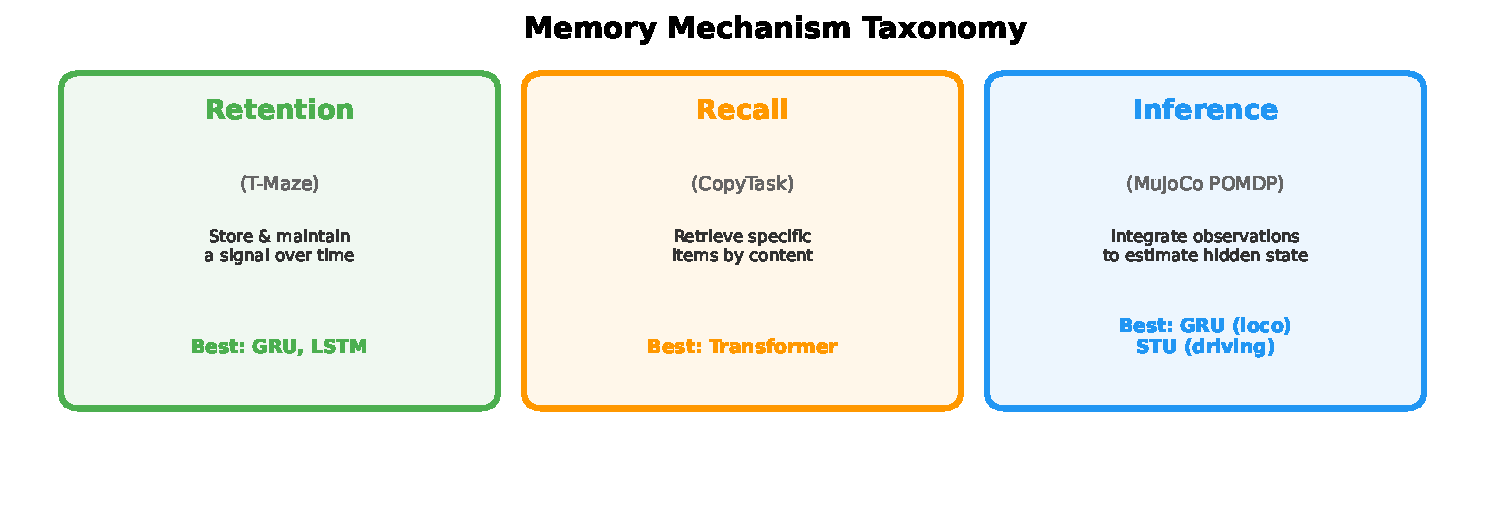
\includegraphics[width=0.85\textwidth]{diagram_taxonomy.pdf}
\caption{Memory mechanism taxonomy. The best architecture depends on the task category, but teacher quality is the dominant factor within each.}
\label{fig:taxonomy}
\end{figure}

Two additional findings deserve note.
First, full STU achieves $5$--$27\times$ lower MSE than GRU on LDS sequence prediction yet does not translate this to distillation, where GRU outperforms STU overall---better sequence prediction does not imply better policy distillation.
Relatedly, the Flash STU tensordot approximation fails catastrophically at compact scale ($d_\text{model}{=}64$), destroying the spectral prior through rank-1 Kronecker constraints.
This is unreported in prior work and directly actionable for practitioners.
Second, self-supervised JEPA provides no benefit for temporal models (likely due to unstable prediction targets), and teacher-supervised JEPA offers only marginal improvement.

\begin{figure}[ht]
\centering
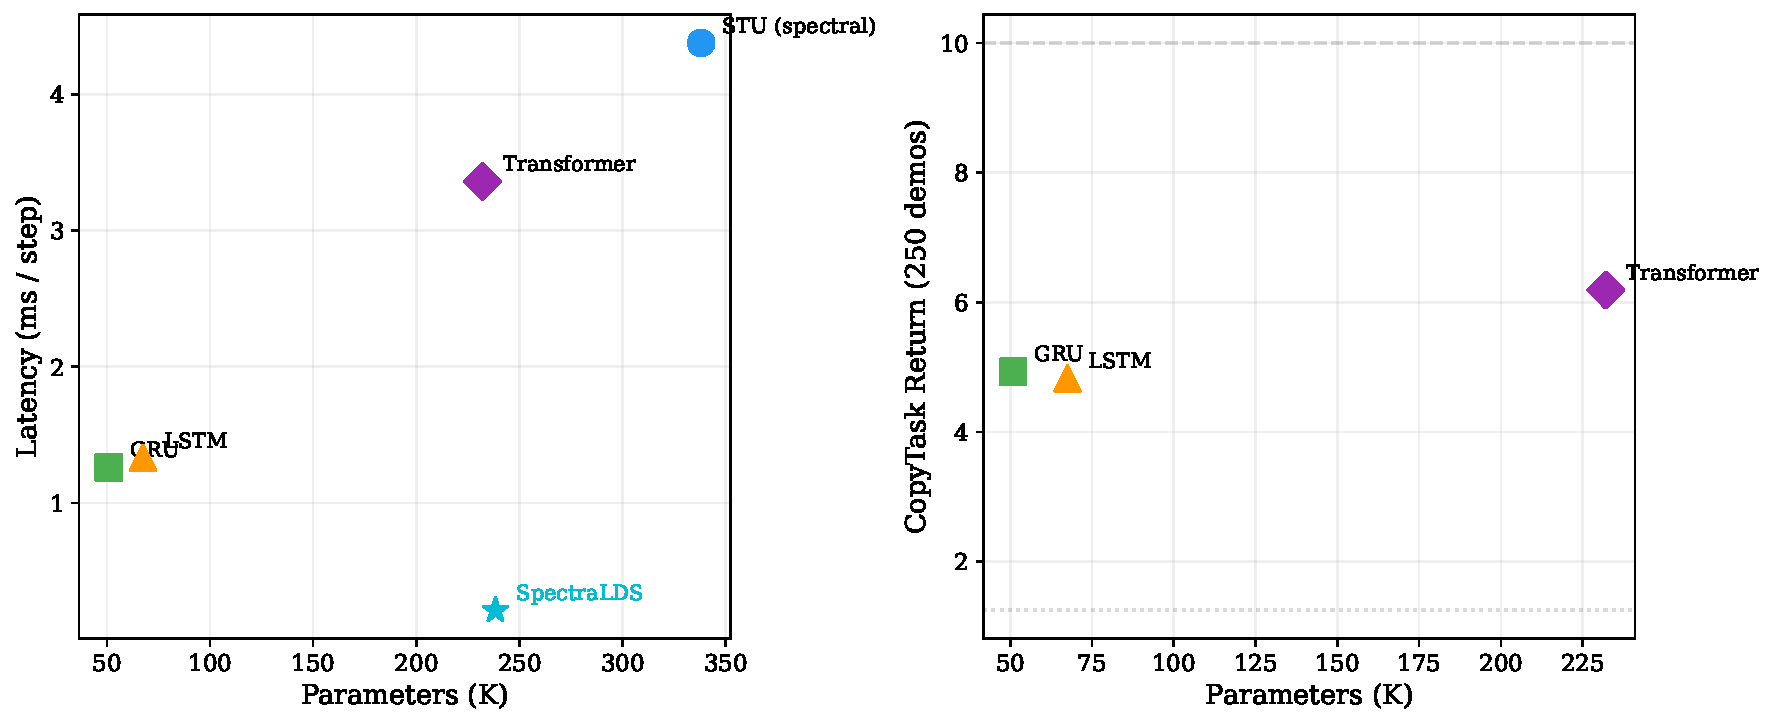
\includegraphics[width=0.65\textwidth]{FIGURE_5_deployment_scatter.pdf}
\caption{Deployment trade-off: parameter count vs.\ inference latency. GRU and LSTM occupy the Pareto-optimal region (low latency, compact). SpectraLDS conversion of a trained STU yields a $16.3\times$ speedup at 0.04\% reconstruction error, making spectral models competitive at deploy time.}
\label{fig:deployment}
\end{figure}

\paragraph{Practical recommendations.}
For practitioners building compact policies via distillation: (1)~invest compute in teacher quality---across our experimental ranges, its $\eta^2$ is $4$--$16\times$ larger than architecture's, though the mean-range ratio is a more conservative $1.7$--$2.5\times$; (2)~use GRU as the default for locomotion and control (51K params, 1.26\,ms latency, most robust); (3)~use Transformer only for content-addressable recall tasks; (4)~consider STU or Transformer for spatially structured observations (lidar, radar); (5)~use full STU, not tensordot, below $d_\text{model}{=}128$; (6)~skip JEPA auxiliary losses.

\paragraph{Limitations.}
Our findings are bounded by several design choices.
We tested only compact models ($d_\text{model}{=}64$, ${\leq}338$K params); at larger scales, the architecture-agnostic story may break as Transformer capacity stops being a liability.
All MuJoCo teachers use a single LSTM-based RecurrentPPO seed; the Ant 2M checkpoint is pathologically unstable, and several striking results (students dramatically exceeding teachers, GRU's large advantage) are driven by this single condition.
With $N{=}3$ seeds on most conditions, the standard error on architecture-level means is of similar magnitude to some reported architecture differences; the teacher quality effect survives this noise (consistent with \citet{belkhale2023data}, who showed data quality dominates other factors in imitation learning) but the architecture ranking does not resolve definitively.
Our MetaDrive results show that the ``GRU is the robust default'' recommendation does not generalize to all task domains---on driving, STU and Transformer lead.
We use only offline behavioral cloning with Gaussian action noise; online distillation (DAgger; \citet{ross2011dagger}) and systematic demonstration biases (as in human demonstrations) may interact differently with architecture choice.
Our POMDP construction (velocity masking) produces a specific kind of partial observability---smooth, continuous hidden state that is approximately a linear function of recent observations. Real-world POMDPs involve occlusions, sensor noise, and discrete mode changes that may interact differently with architecture choice.
Our LSTM teacher creates a potential architecture-matching confound: LSTM students distill from an LSTM-based teacher, which could provide implicit advantages in matching output distributions. The fact that GRU still outperforms LSTM despite this disadvantage strengthens the GRU finding, but we cannot rule out that the ranking would change with a Transformer or spectral teacher.
The $\eta^2$ values characterize variance decomposition over the specific factor ranges we manipulated (teacher return varied ${\sim}7\times$; architecture compared at fixed $d_\text{model}$), and should not be interpreted as universal constants.
The proposed mechanism for students exceeding teachers (variance averaging + length-proportional loss weighting) is consistent with our data but has not been causally tested.

\paragraph{Future work.}
The most impactful extensions are: (1)~an episode-length-normalized BC ablation to causally test the timestep-weighting mechanism; (2)~multi-seed teachers to resolve single-seed artifacts; (3)~a $d_\text{model}$ scaling sweep to test whether teacher-quality dominance persists at larger model scales; (4)~pixel-based POMDPs to test the taxonomy on high-dimensional observations; and (5)~a Transformer teacher to test whether architecture-matched distillation changes the rankings.

All code, experiment scripts, and results are available at \url{https://github.com/wasumayan/wasumind}.
